% \documentclass[aip,jcp,preprint,unsortedaddress,a4paper,onecolum]{revtex4-1}
\documentclass[aip,jcp,a4paper,reprint,onecolumn]{revtex4-1}
% \documentclass[aps,pre,twocolumn]{revtex4-1}
% \documentclass[aps,jcp,groupedaddress,twocolumn,unsortedaddress]{revtex4}

\usepackage[fleqn]{amsmath}
\usepackage{amssymb}
\usepackage[dvips]{graphicx}
\usepackage{color}
\usepackage{tabularx}
\usepackage{algorithm}
\usepackage{algorithmic}

\makeatletter
\makeatother

\newcommand{\recheck}[1]{{\color{red} #1}}
\newcommand{\redc}[1]{{\color{red} #1}}
\newcommand{\bluec}[1]{{\color{blue} #1}}
\newcommand{\vect}[1]{\textbf{\textit{#1}}}
\newcommand{\dd}{\textsf{d}}
\newcommand{\inv}{\textrm{inv}}

\newcommand{\mh}{\mathcal H}
\newcommand{\ml}{\mathcal L}
\newcommand{\mt}{\mathcal T}
\newcommand{\mo}{\mathcal O}
\newcommand{\mi}{\mathcal I}
\newcommand{\mc}{\mathcal C}
\newcommand{\proj}{\mathit\Pi}
\newcommand{\fwg}{{\mathcal A}}
\newcommand{\bwg}{{\mathcal B}}
\newcommand{\bsigma}{\boldsymbol\sigma}


\begin{document}

\title{Linear response theory for core set identification}
\author{Han Wang}
% \affiliation{Institute for Mathematics, Freie Universit\"at Berlin, Germany}
\author{Christof Sch\"utte}
\affiliation{Institute for Mathematics, Freie Universit\"at Berlin, Germany}
% \affiliation{Institute for Mathematics, Freie Universit\"at Berlin, Germany}

\date{\today}

\begin{abstract}
  % In this draft, we are trying to study the core set based Markov
  % State Model (MSM) under non-equilirbium conditions.
\end{abstract}

\maketitle

\section{Perturbation from equilibrium state}
\subsection{The linear response theory}
In this sub-section, we give a brief description of the linear response
theory, for details see Ref.~\cite{tuckeman2010statistical} for
example. Here we assume the system is governed by the
perturbed Langevin equation:
\begin{align}\label{eqn:langevin-1}
  \dot{\vect q} & = \nabla_{\vect p}\mh(\vect q,\vect p)
  + \vect C(\vect q,\vect p) F_e(t)\\\label{eqn:langevin-2}
  \dot{\vect p} & =- \nabla_{\vect q}\mh(\vect q,\vect p)
  + \vect D(\vect q,\vect p) F_e(t)
  - \gamma\vect p
  + \sigma\dot{\vect W}
\end{align}
Where $\vect C$ and $\vect D$ are perturbations to the system, and
$F_e(t)$ is the strength of the perturbation as a function of time,
and is of order $\mo (\varepsilon)$, where $\varepsilon$ is assumed to be small.
The phase space incompressibility condition is assumed:
\begin{align}
  \nabla_{\vect q}\cdot\vect C + \nabla_{\vect p}\cdot\vect D = 0
\end{align}
Then the phase space distribution $f(\vect x, t)$ ($\vect x = \{\vect
q, \vect p\}$) is subject to the Kolmogorov forward equation:
\begin{align}\label{eqn:orig-forward}
  \frac{\partial}{\partial t} f(\vect x, t) - \fwg^\beta(t) f(\vect x, t) = 0
\end{align}
where $\fwg^\beta(t)$ is the forward infiniesimal generator given by
\begin{align}
  \fwg^\beta(t) =
  \frac{\sigma^2}2\Delta_{\vect p}
  - \Big(
  \nabla_{\vect p}\mh + \vect C F_e(t)
  \Big)\cdot\nabla_{\vect q}
  - \Big(
  -\nabla_{\vect q}\mh +
  \vect D F_e(t) - \gamma\vect p
  \Big)\cdot\nabla_{\vect p}
  + 3N\gamma,
\end{align}
and $\beta$ is the inverse temperature.
The fluctuation-dissipation relation is always true:
$\beta = 2\gamma / \sigma^2$.
The equilibrium and unperturbed system
is governed by
the standard Langevin equation, i.e. with
vanishing input perturbation $F_e(t) = 0$ in
Eqn.~\eqref{eqn:langevin-1} and \eqref{eqn:langevin-2}.
We assume that the perturbation to the
system is so small that both the phase space distribution and the
infiniesimal generator can be viewed as perturbation from the initial
distribution and the unperturbed operator
($\vect C = \vect D = 0$),
respectively. We the expansion with respect to small
variable $\varepsilon$:
\begin{align}\label{eqn:f-expan}
  f(\vect x, t) &= f_0(\vect x, t) + \varepsilon f_1(\vect x, t)
  +\varepsilon^2 f_2(\vect x, t) + \mo (\varepsilon^3),
\end{align}
and 
\begin{align}\label{eqn:A-expan}
  \fwg^\beta(t) = \fwg^\beta_0 + \varepsilon\fwg_1(t),
\end{align}
where
\begin{align}
  \fwg_0^\beta =&
  \frac{\sigma^2}2\Delta_{\vect p}
  -
  \nabla_{\vect p}\mh\cdot\nabla_{\vect q}
  - \big(
  -\nabla_{\vect q}\mh - \gamma\vect p
  \big)\cdot\nabla_{\vect p}
  + 3N\gamma,\\
  \fwg_1(t) =&
  - \frac{F_e(t)}{\varepsilon} \big(
  \vect C \cdot\nabla_{\vect q}
  +
  \vect D \cdot\nabla_{\vect p}
  \big).
\end{align}
Notice $F_e(t) \sim \mo(\varepsilon)$, so $\Vert\fwg_1(t)\Vert\sim\mo(1)$.
The invariant measure of $\fwg^\beta_0$ satisfies $\fwg^\beta_0f^\beta_{\inv}(\vect x) = 0$,
which is nothing but the Boltzmann distribution
\begin{align}
  f^\beta_{\inv}(\vect x) \propto e^{-\beta\mh(\vect x)}
\end{align}
Inserting \eqref{eqn:f-expan} and \eqref{eqn:A-expan} into
\eqref{eqn:orig-forward}, 
the Kolmogorov forward equation becomes:
\begin{align}
  \frac{\partial}{\partial t}
  [f_0(\vect x, t) + \varepsilon  f_1(\vect x, t) + \varepsilon^2f_2(\vect x, t)]
  -
  [\,\fwg^\beta_0 + \varepsilon\fwg_1(t)\,]
  [f_0(\vect x, t) + \varepsilon  f_1(\vect x, t) + \varepsilon^2f_2(\vect x, t)]
  = 0
\end{align}
Matching this equation at different orders of $\varepsilon$, the zeroth
order gives:
\begin{align}\label{eqn:e-o0}
  \bigg[
  \frac{\partial}{\partial t}
  - \fwg_0^\beta
  \bigg]
  f_0(\vect x, t)
  = 0
\end{align}
which is the unperturbed equation. Matching the first and the second order gives:
\begin{align}\label{eqn:e-o1}
  \bigg[
  \frac{\partial}{\partial t}
  - \fwg_0^\beta
  \bigg]
  f_1(\vect x, t)
  =&
  \fwg_1(t) f_0(\vect x, t)\\\label{eqn:e-o2}
  \bigg[
  \frac{\partial}{\partial t}
  - \fwg_0^\beta
  \bigg]
  f_2(\vect x, t)
  =&
  \fwg_1(t) f_1(\vect x, t)
\end{align}
Formally solving \eqref{eqn:e-o0} -- \eqref{eqn:e-o2} with
inital conditions $f_1(\vect x, 0) = 0$ and $f_2(\vect x, 0) = 0$
gives
\begin{align}\label{eqn:f0-0}
  f_0(\vect x, t)
  =&\,
  e^{t\fwg^\beta_0}f_0(\vect x, 0) \\\label{eqn:f1-0}
  f_1(\vect x, t)
  =&\,
  \int_0^t\dd s\,
  e^{(t-s)\fwg^\beta_0}\circ
  \fwg_1(s) f_0(\vect x,s)
  =
  \int_0^t\dd s\,
  e^{(t-s)\fwg^\beta_0}\circ
  \fwg_1(s)\circ
  e^{s\fwg^\beta_0}f_0(\vect x, 0) \\\nonumber
  f_2(\vect x, t)
  =&\,
  \int_0^t\dd s\,
  e^{(t-s)\fwg^\beta_0}\circ
  \fwg_1(s) f_1(\vect x,s) \\\label{eqn:f2-0}
  &=
  \int_0^t\dd s
  \int_0^s\dd u\,\,
  e^{(t-s)\fwg^\beta_0}\circ
  \fwg_1(s)\circ
  e^{(s-u)\fwg^\beta_0}\circ
  \fwg_1(u)\circ
  e^{u\fwg^\beta_0}
  f_0(\vect x, 0) 
\end{align}
If the initial distribution is the invariant distribution, i.e.
$f_0(\vect x, 0) = f_{\inv}^\beta(\vect x)$,
\eqref{eqn:f0-0} becomes:
\begin{align}
  f_0(\vect x, t) = f_{\inv}^\beta(\vect x)
\end{align}
It can be shown that
\begin{align}
  \fwg_1(s) f_{\inv}^\beta(\vect x)
  =
  -\frac{F_e(s)}{\varepsilon}\beta
  j(\vect x)
  f_{\inv}^\beta(\vect x),
\end{align}
where the \emph{dissipative flux} $j(\vect x)$ is defined by,
\begin{align}
  j(\vect x) =
  -\vect C\cdot\nabla_{\vect q}\mh 
  -\vect D\cdot\nabla_{\vect p}\mh
\end{align}
Then $f_1(\vect x, t)$ becomes:
\begin{align}
  f_1(\vect x, t)
  =
  -\frac\beta\varepsilon
  \int_0^t\dd s\,
  F_e(s)\,
  e^{(t-s)\fwg^\beta_0}
  \big[
  j(\vect x)
  f_{\inv}^\beta(\vect x)
  \big]
\end{align}
Therefore, the linear order approximation to
the solution of~\eqref{eqn:orig-forward} is 
\begin{align}\label{eqn:solv-orig-linear}
  f(\vect x, t) =
  f_{\inv}^\beta(\vect x)
  - \beta
  \int_0^t\dd s\,
  F_e(s)\,
  e^{(t-s)\fwg^\beta_0}
  \big[
  j(\vect x)
  f_{\inv}^\beta(\vect x)
  \big]
  + \mo(\varepsilon^2)
\end{align}
For any time-dependent observation, the linear response approximation
would be:
\begin{align}\nonumber
  \mathcal O(t)
  &=
  \int\dd \vect x \:O(\vect x)f(\vect x, t)  \\\nonumber
  &=
  \int\dd \vect x\, O(\vect x)\,
  [\,f_{\inv}^\beta(\vect x) + \varepsilon f_1(\vect x, t)] \\\nonumber
  &=
  \langle O\rangle
  -
  \beta
  \int \dd \vect x\:
  O(\vect x)
  \int_0^t\dd s\,F_e(s)
  e^{(t-s)\fwg_0^\beta}
  \big[j(\vect x)f^\beta_{\inv}(\vect x)\big]
  \\\nonumber
  &=
  \langle O\rangle
  -
  \beta
  \int_0^t\dd s\,
  F_e(s)
  \int \dd \vect x\,
  O(\vect x)\,
  e^{(t-s)\fwg_0^\beta}
  \big[j(\vect x)f^\beta_{\inv}(\vect x)\big]
  \\\nonumber
  &=
  \langle O\rangle
  -
  \beta
  \int_0^t\dd s\,
  F_e(s)
  \int \dd \vect x\,
  f^\beta_{\inv}(\vect x) j(\vect x)\,
  e^{(t-s)\bwg^\beta_0}
  O(\vect x)\\ \label{eqn:eqi-pert-1}
  &=
  \langle O\rangle
  -
  \beta
  \int_0^t\dd s\,
  F_e(t-s)
  \int \dd \vect x\,
  f^\beta_{\inv}(\vect x) j(\vect x)\,
  e^{s\bwg_0^\beta}
  O(\vect x)
\end{align}
Where $\bwg^\beta_0$ is the infiniesimal generator of the \emph{unperturbed} 
Kolmogorov backward equation, which is the adjoint operator of $\fwg^\beta_0$.
We have
\begin{align}
  e^{s\bwg^\beta_0} O(\vect x) = \mathbb E_{\vect x} [O(\vect X^\beta_s)]
\end{align}
where $\vect X^\beta_t$ is the trajectory of the unperturbed Langevin equation
starting at $\vect x$.
Therefore, we have
% Notice that $e^{i\ml_0(t-s)}O(\vect x) = O(\phi_{t-s}(\vect x))$,
% where $\phi_t(\vect x)$ is the flow mapping of the \emph{unperturbed}
% Hamiltonian system. We have
\begin{align}
  \mathcal O(t)
  =
  \langle O\rangle
  -
  \beta
  \int_0^t\dd s\,
  F_e(t-s)
  \int \dd \vect x\,
  f^\beta_{\inv}(\vect x)
  j(\vect x)\,
  \mathbb E_{\vect x} [O(\vect X^\beta_s)]
\end{align}
or equivalently:
\begin{align}\label{eqn:lr}
  \mathcal O(t)
  =
  \langle O\rangle
  -
  \beta
  \int_0^t\dd s\,
  F_e(t-s)
  \big\langle
  j(0)\,
  \mathbb E_{\vect x} [O(\vect X^\beta_s)]
  \big\rangle
\end{align}
where $  \langle
  j(0)\,
  \mathbb E_{\vect x} [O(\vect X^\beta_s)]
  \rangle$ is the \emph{equilibrium time
  correlation} between the observation $O$ at time $s$ and the
dissipative flux $j$.


\subsection{The linear response theory for the core set identification}

The core set plays a very important role in the MSM theory. One way to
identify core set is to consider the ``stability'' of the invariant
measure $f^\beta_{\inv}$ under a propagator $\mt_\tau$
of time step $\tau$.
For example, the propagator is chosen $\mt_\tau = e^{\tau\fwg_t^{2\beta}}$,
i.e. integrating the Langevin equation~\eqref{eqn:langevin-1}
and \eqref{eqn:langevin-2} at temperature $1/2\beta$ for time $\tau$.
Notice $\tau$ is an artificial time that is ``orthogonal'' to the real
time $t$.
% , which is associated with a
% stochastic process denoted by $\vect Y_\alpha$:
The core set is identified by:
\begin{align}
  C_\tau(t) = \big\{
  \vect x \,\vert\, \mt_\tau f(\vect x, t) > f(\vect x, t)
  \big\}
\end{align}
Generally, it is impossible and not necessary to consider the core set
in the $3N$ dimensional configuration space. For example, a
macromolecule solving in water, the DOFs of water is not of interest
at all. Therefore, we consider some phase space compressing function
$\vect y = \vect y(\vect x)$, with $\vect y \in \Omega \subset \mathbb
R^M,\ M\ll 3N$. We call $\Omega$ the observation space.  The projected
invariant measure on the observation space is therefore
\begin{align}
  \proj f (\vect y, t)
  =
  \int
  \dd \vect x\,
  f(\vect x, t) \,
  \delta (\vect y - \vect y(\vect x)) 
\end{align}
The core set on the observation space is
\begin{align}
  \widetilde
  C_\tau(t) = \big\{
  \vect y \,\vert\,
  \proj\mt_\tau f(\vect y, t) > \proj f(\vect y, t)
  \big\}
\end{align}
% with $\widetilde \mt_\alpha$ defined by
% $\widetilde\mt_\alpha = \mathcal P\circ\mt_\alpha$, namely
% \begin{align}
%   \widetilde\mt_\alpha\, p_0(\vect y)
%   =
%   \mathcal P\circ\mt_\alpha f_0 (\vect y)
%   =
%   \int
%   \dd \vect x\,
%   [\mt_\alpha f_0](\vect x) \,
%   \delta (\vect y - \vect y(\vect x)) 
% \end{align}
For convenience, we define $\Delta \mt_\tau =
\mt_\tau - \mathcal I$, where $\mathcal I$ is the
identity. If $[\proj\circ\Delta \mt_\tau f](\vect y, t) > 0$, then
$\vect y$ is in the core set $\widetilde C_\tau(t) $.
\begin{align}\nonumber
  [\proj\circ\Delta \mt_\tau f](\vect y, t)
  &=
  \int
  \dd \vect x\,
  \Delta \mt_\tau f(\vect x, t) \,
  \delta (\vect y - \vect y(\vect x))  \\\nonumber
  &=
  \lim_{\sigma \rightarrow 0}
  \int
  \dd \vect x\,
  \Delta \mt_\tau f(\vect x, t) \,
  K_{\sigma} (\vect y - \vect y(\vect x))  \\\label{eqn:core-identify}
  &=
  \lim_{\sigma \rightarrow 0}
  \int
  \dd \vect x\,
  \Delta \mt_\tau f(\vect x, t) \,
  K_{\sigma, \vect y} (\vect x)
  % \\\nonumber
  % &=
  % \lim_{\sigma \rightarrow 0}
  % \int
  % \dd \vect x\,
  % f_0(\vect x) \,
  % [\Delta \mt_\alpha]^\dagger K_{\sigma, \vect y} (\vect x)\\
  % &=
  % \lim_{\sigma \rightarrow 0}\,
  % \langle
  % [\Delta \mt_\alpha]^\dagger K_{\sigma, \vect y}
  % \rangle_0
\end{align}
For convenience, we denote $f_t(\vect x) = f(\vect x, t)$.
Notice that $\mt_\tau f_t(\vect x) = e^{\tau \fwg_t^{2\beta}} f_t(\vect x)$
is the solution of
\begin{align}
  \frac{\partial}{\partial \tau} f_t(\vect x, \tau)
  -
  \fwg^{2\beta}(t)  f_t(\vect x, \tau)
  =0
\end{align}
with inital condition $f_t(\vect x, \tau = 0) = f_t(\vect x)$. We do the same
expansion as before, and then
matching different orders of $\varepsilon$ gives:
\begin{align}
  &\bigg[
  \frac{\partial}{\partial \tau}
  - \fwg_0^{2\beta}
  \bigg]
  f_{t,0}(\vect x, \tau)
  = 0 \\
  &\bigg[
  \frac{\partial}{\partial \tau}
  - \fwg_0^{2\beta}
  \bigg]
  f_{t,1}(\vect x, \tau)
  =
  \fwg_1(t) f_{t,0}(\vect x, \tau)
\end{align}
Formally solving these equations with
inital conditions $f_{t,0}(\vect x, 0) = f_t(\vect x) = f(\vect x, t)$
and  $f_{t,1}(\vect x, 0) = 0$ 
gives
\begin{align}\label{eqn:f0-1}
  f_{t,0}(\vect x, \tau)
  =&\,
  e^{\tau\fwg^{2\beta}_0}f_{t,0}(\vect x, 0) \\\label{eqn:f1-1}
  f_{t,1}(\vect x, \tau)
  =&\,
  \int_0^\tau\dd \eta\,
  e^{(\tau-\eta)\fwg^{2\beta}_0}\circ
  \fwg_1(t) f_{t,0}(\vect x,\eta)
  =
  \int_0^\tau\dd \eta\,
  e^{(\tau-\eta)\fwg^{2\beta}_0}\circ
  \fwg_1(t)\circ
  e^{\eta\fwg^{2\beta}_0}f_{t,0}(\vect x, 0) 
\end{align}
By inserting the linear order approximated solution~\eqref{eqn:solv-orig-linear}
in to the above equations, we have:
\begin{align}\nonumber
  \mt_\tau f_t(\vect x)=
  f_{t}(\vect x, \tau)
  =&\,
  e^{\tau\fwg^{2\beta}_0} f_{\inv}^\beta(\vect x) -
  \beta
  \int_0^t\dd s\,
  F_e(s)\,
  e^{\tau\fwg^{2\beta}_0} \circ
  e^{(t-s)\fwg^\beta_0}
  \big[
  j(\vect x)
  f_{\inv}^\beta(\vect x)
  \big]
  \\\label{eqn:solve-tau-linear}
  &\,+ \varepsilon
  \int_0^\tau\dd \eta\,
  e^{(\tau-\eta)\fwg^{2\beta}_0}\circ
  \fwg_1(t)\circ
  e^{\eta\fwg^{2\beta}_0}f_{\inv}^\beta(\vect x)  + \mo(\varepsilon^2)
\end{align}
By inserting~\eqref{eqn:solv-orig-linear} and~\eqref{eqn:solve-tau-linear}
into~\eqref{eqn:core-identify}, we have, up to the first order
approximation,
\begin{align}\nonumber
  [\proj\circ\Delta\mt_\tau f](\vect y, t)
  \approx
  \lim_{\sigma \rightarrow 0}
  \bigg\{
    &\,
    \int \dd \vect x\,
    \big(e^{\tau\fwg_0^{2\beta}}-\mi\big)
    f_{\inv}^\beta(\vect x)\,
    K_{\sigma,\vect y}(\vect x)\\\nonumber
    &
    - \int_0^t\dd s\,
    F_e(s)
    \int\dd \vect x\,
    \big(e^{\tau\fwg^{2\beta}_0} - \mi\big)\circ
    e^{(t-s)\fwg^\beta_0}
    \big[
    j(\vect x)
    f_{\inv}^\beta(\vect x)
    \big]\, K_{\sigma,\vect y}(\vect x) \\\nonumber
    &
    +
    \varepsilon
    \int_0^\tau\dd \eta
    \int\dd \vect x\,
    e^{(\tau-\eta)\fwg^{2\beta}_0}\circ
    \fwg_1(t)\circ
    e^{\eta\fwg^{2\beta}_0}f_{\inv}^\beta(\vect x)\,K_{\sigma,\vect y}(\vect x)
    \bigg\}     \\\nonumber
  \approx
  \lim_{\sigma \rightarrow 0}
  \bigg\{
  &\,
    \Big\langle
    \mathbb E_{\vect x}[ K_{\sigma,\vect y}(\vect X^{2\beta}_\tau) ]
    - K_{\sigma,\vect y}(\vect x)
    \Big\rangle\\\nonumber
    &
    - \int_0^t\dd s\,
    F_e(s)
    \Big\langle
    j(\vect x)\,
    \mathbb E_{\vect x}\big\{
    \mathbb E_{\vect X_{t-s}^\beta}[
    K_{\sigma,\vect y}(\vect X_\tau^{2\beta})
    ]
    -
    K_{\sigma,\vect y}(\vect X_{t-s}^\beta)
    \big\}
    \Big\rangle\\\label{eqn:core-identify-approx-1}
    &
    +
    \varepsilon
    \int_0^\tau\dd \eta
    \int\dd \vect x\,
    e^{(\tau-\eta)\fwg^{2\beta}_0}\circ
    \fwg_1(t)\circ
    e^{\eta\fwg^{2\beta}_0}f_{\inv}^\beta(\vect x)\,K_{\sigma,\vect y}(\vect x)
    \bigg\}     
\end{align}
Unfortunately the last term on the r.h.s. of~\eqref{eqn:core-identify-approx-1}
is not easy to calculate. We will deal with it with
the path integral method introduced later.




\subsection{Path integral}
The path integral is very useful to develop the non-equilibrium version of
linear response theory. 
Comparing with the idea of ensemble, which is a collection of state points
in the configuration space, the path integral consider the ``ensemble'' of
trajectories.
(In the following, the develop of formula are formal. The strict mathematical
theory is still unclear for me.)
First, we take the standard 1-dimensional Wiener process for example.
Consider the time interval $[0,T]$, the probability density of one trajectory
is given by
\begin{align}
  p[W_t] = \frac 1Z e^{-I[W_t]}
\end{align}
where $I$ is the action functional of Wiener process given by
\begin{align}
  I[W_t] = \int_0^T\frac12 \dot{W}_t^2\dd t
\end{align}
the partition function $Z$ is
\begin{align}
  Z = \int  e^{-I[W_t]} \prod_{0\leq t\leq T}\dd W_t
\end{align}
Consider the following two stochastic processes:
\begin{align}\label{eqn:st-orig}
  \dd \vect X_t &= \vect b(\vect X_t, t) \dd t + \bsigma(\vect X_t, t)\,\dd\vect W_t \\\label{eqn:st-pert}
  \dd \vect Y_t &= \vect b(\vect Y_t, t) \dd t + \vect c(\vect Y_t, t) \dd t + \bsigma(\vect Y_t, t)\,\dd\vect W_t
\end{align}
Where $\vect W_t$ is the standard Wiener process. Obviously
\eqref{eqn:st-pert} is the perturbed version of
\eqref{eqn:st-orig}. It has been shown that, starting from the same
measure saying $\mu$ (which is not necessarily equilibrium or
stationary), the ratio of trajectory probability density between the perturbed
and unperturbed process is~\cite{li2010lecture} (\recheck{I think here
  the incompressibility of phase space should be assumed. Otherwise the
  ratio should be more complicated.})
\begin{align}\label{eqn:girsanov}
  \frac{\dd\mathcal P_{\vect Y}}{\dd\mathcal P_{\vect X}}
  =
  \exp
  \Big\{
  -\frac12 \int_0^T\vert\bsigma^{-1}\cdot\vect c(\vect X_t,t)\vert^2\,\dd t
  +\int_0^T[\dot{\vect X}_t - \vect b(\vect X_t,t)]^T
  \cdot\bsigma^{-T}\cdot\bsigma^{-1}\cdot\vect c(\vect X_t,t)\,\dd t 
  \Big\}
\end{align}
where $\mathcal P_{\vect Y}$ and $\mathcal P_{\vect Y}$ are measures
of the trajectories generated by \eqref{eqn:st-pert} and
\eqref{eqn:st-orig}, respectively.  This result (Girsanov formula?) is
(formally) precise without any approximation.


To be more general, we study the two perturbed Langevin dynamics
(i.e. Eqn.~\eqref{eqn:langevin-1} and \eqref{eqn:langevin-2}) with
different perturbations that are given by $F_e^1(t)$ and $F_e^2(t)$,
respectively. 
By writing Eqn.~\eqref{eqn:langevin-1} and \eqref{eqn:langevin-2} as
\begin{align}
  \left[
    \begin{array}{l}
      \dd\vect q\\
      \dd\vect p
    \end{array}
  \right]
  =
  \left[
    \begin{array}{l}
      \nabla_{\vect p}\mh\\
      -\nabla_{\vect q}\mh - \gamma\vect p + F_e\vect D
    \end{array}
  \right]
  \dd t
  +
  \left[
    \begin{array}{cc}
      \epsilon \vect I & 0\\
      0 & \sigma\vect I
    \end{array}
  \right]
  \cdot
  \left[
    \begin{array}{l}
      \dd\vect W_t\\
      \dd\vect W_t
    \end{array}
  \right]
\end{align}
Using Girsanov's formula, to the leading order of $\Delta F_e = F_e^2 - F_e^1$,
we have
\begin{align}\label{eqn:girsanov-1}
  \frac{\dd\mathcal P^2[\vect X_t]}{\dd\mathcal P^1[\vect X_t]}
  &=
  \exp
  \Big\{
  \frac 1 {\sigma^2}
  \int_0^t
  [\dot{\vect p}_s +
  \gamma\vect p_s +
  \nabla_{\vect q}\mh(\vect q_s,\vect p_s)
  - F_e^1(s) \vect D(\vect q_s,\vect p_s)
  ]\cdot
  \vect D(\vect q_s,\vect p_s)
  \Delta F_e(s)\,
  \dd s
  + \mathcal O(\Delta F_e^2)
  \Big\} 
\end{align}





\subsection{The linear response theory for the core set identification,
  revisited by the path integral}
For some observable $O[\vect X_\eta]$, which is a functional of the
stochastic process $\vect X_\eta$,
the trajectory ensemble average yields:
\begin{align}
  \mo(t)
  =
  \int \dd \mu_t(\vect x)
  \int_{\mc\{\vect x,0;\tau\}}
  O[\vect X_\eta]\,
  \dd \mathcal P^{2\beta}_t[\vect X_\eta],
\end{align}
where $\mu_t(\vect x)$
is the measure of the initial position, and obviously, we have
$\dd \mu_t(\vect x) = f_t(\vect x)\,\dd \vect x$.
The trajectory $\vect X_\eta \in {\mc\{\vect x,0;\tau\}}$, where
${\mc\{\vect x,0;\tau\}}$ denotes the set of all continuous but not
differentiable trajectories starting at $\vect x$ at artificial
time 0, and ending
at artificial time $\tau$.
$\mathcal P^{2\beta}_t$ denotes the measure of trajectories
developped under temperature $1/2\beta$
at real time $t$.
Since the perturbation is a function of time, this
measure also depends on time. The reference artificial dynamics is chosen
at $t=0$.
In this case, \eqref{eqn:girsanov-1} rewrites:
\begin{align}\nonumber
  \frac{\dd \mathcal P^{2\beta}_t[\vect X_\eta]}
  {\dd \mathcal P^{2\beta}_0[\vect X_\eta]}\,
  &=
  \exp
  \Big\{
  \frac 1 {\sigma^2}
  \int_0^\tau
  [\dot{\vect p}_\eta +
  \gamma\vect p_\eta +
  \nabla_{\vect q}\mh(\vect q_\eta,\vect p_\eta)
  ]\cdot
  \vect D(\vect q_\eta,\vect p_\eta)
  F_e(t)\,
  \dd \eta
  + \mathcal O(\varepsilon^2)
  \Big\}\\
  &=
  1+
  F_e(t)\,
  \frac 1 {\sigma^2}
  \int_0^\tau
  [\dot{\vect p}_\eta +
  \gamma\vect p_\eta +
  \nabla_{\vect q}\mh(\vect q_\eta,\vect p_\eta)
  ]\cdot
  \vect D(\vect q_\eta,\vect p_\eta)\,
  \dd \eta
  + \mathcal O(\varepsilon^2)  
\end{align}
Notice that $F_e(t)\sim \mo(\varepsilon)$.
For convenience, we denote
\begin{align}
  G[\vect X_\eta] &=
    \frac 1 {\sigma^2}
  \int_0^\tau
  [\dot{\vect p}_\eta +
  \gamma\vect p_\eta +
  \nabla_{\vect q}\mh(\vect q_\eta,\vect p_\eta)
  ]\cdot
  \vect D(\vect q_\eta,\vect p_\eta)\,
  \dd \eta =
  \frac1\sigma\int_0^\tau
  \vect D(\vect q_\eta,\vect p_\eta)
  \cdot\dd \vect W_\eta
\end{align}
where $\vect W_\eta$ is the Wiener process that generates
$\vect X_\eta$.
Therefore, we have
\begin{align}\nonumber
  \mo(t)
  =&\,
  \int \dd \vect x
  f(\vect x, t)
  \int_{\mc\{\vect x,0;\tau\}}
  O[\vect X_\eta]\,
  \frac{\dd \mathcal P^{2\beta}_t[\vect X_\eta]}
  {\dd \mathcal P^{2\beta}_0[\vect X_\eta]}\,
  \dd \mathcal P^{2\beta}_0[\vect X_\eta]  \\\nonumber
  =&\,
  \int \dd \vect x
  \big[
  f_{0}(\vect x, t)
  + \varepsilon f_{1}(\vect x, t)
  + \mo(\varepsilon^2)
  \big]
  \int_{\mc\{\vect x,0;\tau\}}
  O[\vect X_\eta]\,
  \big[
  1 
  + F_e(t) G[\vect X_\eta]
  + \mo(\varepsilon^2)
  \big]
  \dd \mathcal P^{2\beta}_0[\vect X_\eta]
  \\\nonumber
  =&\,
  \int \dd \vect x
  f_{0}(\vect x, t)
  \int_{\mc\{\vect x,0;\tau\}}
  O[\vect X_\eta]\,
  \dd \mathcal P^{2\beta}_0[\vect X_\eta]
  +
  \varepsilon
  \int \dd \vect x\,
  f_{1}(\vect x, t)
  \int_{\mc\{\vect x,0;\tau\}}
  O[\vect X_\eta]\,
  \dd \mathcal P^{2\beta}_0[\vect X_\eta]\\\label{eqn:solve-tau-linear-2-0}
  &+
  F_e(t)
  \int \dd \vect x\,
  f_{0}(\vect x, t)
  \int_{\mc\{\vect x,0;\tau\}}
  O[\vect X_\eta]\,
  G[\vect X_\eta]\,
  \dd \mathcal P^{2\beta}_0[\vect X_\eta]
  + \mo(\varepsilon^2) 
\end{align}
In the case of core set identification,
\begin{align}\nonumber
  [\proj\circ \mt_\tau] f(\vect y,t)
  =&\,
  \int\dd \vect x\,
  \mt_\tau f(\vect x,t) K_{\sigma,\vect y}(\vect x)\\\nonumber
  =&\,
  \int\dd \vect x\,
  e^{\tau\fwg_t^{2\beta}} f(\vect x,t) \,K_{\sigma,\vect y}(\vect x)\\\nonumber
  =&\,
  \int\dd \vect x\,
  f(\vect x,t) \,e^{\tau\bwg_t^{2\beta}}K_{\sigma,\vect y}(\vect x)  \\\nonumber
  =&\,
  \int\dd \vect x\,
  f(\vect x,t) \,\mathbb E_{\vect x}
  \big[
  K_{\sigma,\vect y}(\vect X^{2\beta}_{t,\tau})
  \big]  
  \\
  =&\,
  \int\dd \vect x\,
  f(\vect x,t) 
  \int_{\mc\{\vect x,0;\tau\}} K_{\sigma,\vect y}(\vect X_\tau)\,
  \dd\mathcal P^{2\beta}_t[\vect X_\eta]
\end{align}
So the observable $O[\vect X_\eta]$
is:
\begin{align}
  O[\vect X_\eta] = 
  K_{\sigma,\vect y}(\vect X_\tau),
  % -
  % K_{\sigma,\vect y}(\vect x)
\end{align}
which is the end point of the artificial
trajectory measured by $K_{\sigma,\vect y}$.
Inserting everything we known in~\eqref{eqn:solve-tau-linear-2-0},
and notice $G[\vect X_\eta] = 0$ when $\tau = 0$,
\begin{align}\nonumber
  [\proj\circ\Delta\mt_\tau f](\vect y, t)
  =
  \lim_{\sigma \rightarrow 0}
  \big\{
  &\,
  [\proj\circ\mt_\tau f - \proj\circ\mt_0 f](\vect y, t)
  \big\}\\\nonumber
  \approx
  \lim_{\sigma \rightarrow 0}
  \bigg\{
  &\,
  \int \dd \vect x\,
  f_\inv^\beta(\vect x)
  \int_{\mc\{\vect x,0;\tau\}}
  [K_{\sigma,\vect y}(\vect X_\tau)
  -K_{\sigma,\vect y}(\vect x)]  \,
  \dd \mathcal P^{2\beta}_0[\vect X_\eta]\\\nonumber
  &\,-
  \beta
  \int_0^t\dd s\, F_e(s)
  \int \dd \vect x\,
  e^{(t-s)\fwg_0^\beta}
  \big[
  j(\vect x)
  f_\inv^\beta(\vect x)
  \big]
  \int_{\mc\{\vect x,0;\tau\}}
  [K_{\sigma,\vect y}(\vect X_\tau)
  -K_{\sigma,\vect y}(\vect x)]  \,
  \dd \mathcal P^{2\beta}_0[\vect X_\eta]\\\nonumber
  &\,+
  F_e(t)
  \int \dd \vect x\,
  f_\inv^\beta(\vect x)
  \int_{\mc\{\vect x,0;\tau\}}
  K_{\sigma,\vect y}(\vect X_\tau)
  % \Big\{
  % \int_0^\tau\dd \eta\,
  % [\dot{\vect p}_\eta + \gamma\vect p_\eta + \nabla_{\vect q}\mh(\vect X_\eta)]
  % \cdot\vect D(\vect X_\eta)
  % \Big\}\,
  \,G[\vect X_\eta]\,
  \dd \mathcal P^{2\beta}_0[\vect X_\eta]
  \bigg\}\\\nonumber
  \approx
  \lim_{\sigma \rightarrow 0}
  \bigg\{
  &\,
  \Big\langle
  \mathbb E_{\vect x}[K_{\sigma,\vect y}(\vect X_\tau^{2\beta})]
  -
  K_{\sigma,\vect y}(\vect x)
  \Big\rangle\\\nonumber
  &\,
  - \beta
  \int_0^t\dd s\, F_e(s)
  \Big\langle
  j(\vect x)
  \mathbb E_{\vect x} \big\{
  \mathbb E_{\vect X^\beta_{t-s}}\big[
  K_{\sigma, \vect y}(\vect X^{2\beta}_\tau)
  \big]
  -
  K_{\sigma, y}(\vect X^\beta_{t-s})
  \big\}
  \Big\rangle\\\label{eqn:core-identify-approx-2}
  &\,+
  F_e(t)
  \int \dd \vect x\,
  f_\inv^\beta(\vect x)
  \int_{\mc\{\vect x,0;\tau\}}
  K_{\sigma,\vect y}(\vect X_\tau)
  \,G[\vect X_\eta]\,
  \dd \mathcal P^{2\beta}_0[\vect X_\eta]
  \bigg\}
\end{align}
Comparing~\eqref{eqn:core-identify-approx-2}
with~\eqref{eqn:core-identify-approx-1}, the first
two terms on the r.h.s. are identical. 
The last term is now computable.


\subsection{General response theory for core set identification}

Here, we assume that the system undergoes a series of perturbations,
which are denoted by $F^0_e(t),\ F^1_e(t),\ \cdots,\ F^i_e(t),\ \cdots$.
Here, $F^0_e(t) = 0$.
The measure for the trajectory space
$\mc\{\vect x, 0; t\}$
is given by
$\mathcal P_0^\beta[\vect X_s],\ \mathcal P_1^\beta[\vect X_s],\ \cdots,\
\mathcal P_i^\beta[\vect X_s], \cdots$, respectively.
The measure for the quenching trajectory are denoted by
$\mathcal P_{0,t}^{2\beta}[\vect X_\eta],\
\mathcal P_{1,t}^{2\beta}[\vect X_\eta],\ \cdots,\
\mathcal P_{i,t}^{2\beta}[\vect X_\eta], \cdots$, respectively.
The notation $t$ on the subscript means the trajectory is branched from
the main trajectory at time $t$.
Now the phase space distribution $f_i(\vect x, t)$ for the
$i$-th perturbation can be studied in terms
of path integral:
\begin{align}
  f_i(\vect x, t) =
  \int\dd\vect u\,
  f_i(\vect u, 0)
  \int_{\mc\{\vect u,0; \vect x,t\}}
  \dd\mathcal P_i^\beta[\vect X_s]
\end{align}
Applied by operator $\mt_\tau$, we have
\begin{align}\nonumber
  \mt_\tau f_i(\vect x, t)
  =&\,
  \int\dd\vect u f_i(\vect u, t)
  \int_{\mc\{\vect u,0; \vect x,\tau\}}
  \dd\mathcal P_{i,t}^{2\beta}[\vect X_\eta]\\
  =&\,
  \int\dd\vect v\,
  f_i(\vect v, 0)
  \int\dd\vect u
  \int_{\mc\{\vect v,0; \vect u,t\}}
  \dd\mathcal P_i^\beta[\vect X_s]  
  \int_{\mc\{\vect u,0; \vect x,\tau\}}
  \dd\mathcal P_{i,t}^{2\beta}[\vect X_\eta]
\end{align}
For the core set identification,
\begin{align}
  [\proj\circ\mt_\tau f](\vect y, t)
  &=
  \int\dd\vect v\,
  f_i(\vect v, 0)
  \int\dd\vect u
  \int_{\mc\{\vect v,0; \vect u,t\}}
  \dd\mathcal P_i^\beta[\vect X_s]  
  \int_{\mc\{\vect u,0; \tau\}}
  K_{\sigma,\vect y}(\vect X_\tau)\,
  \dd\mathcal P_{i,t}^{2\beta}[\vect X_\eta]  \\
  [\proj\circ\mt_0 f](\vect y, t)
  &=
  \int\dd\vect v\,
  f_i(\vect v, 0)
  \int_{\mc\{\vect v,0; t\}}
  K_{\sigma,\vect y}(\vect X_t)\,
  \dd\mathcal P_i^\beta[\vect X_s]  
  % \int_{\mc\{\vect u,0; \tau\}}
  % K_{\sigma,\vect y}(\vect X_\tau)\,
  % \dd\mathcal P_{i,t}^{2\beta}[\vect X_\eta]  
\end{align}
Here we assume that the system always starts from invariant measure,
i.e. $f_i(\vect x, 0) = f_{\inv}^\beta(\vect x)$, and that we have a
good sampling of the $(i-1)$-th perturbation, then
\begin{align}
  [\proj\circ\mt_\tau f](\vect y, t)
  &=
  \int\dd\vect v\,
  f_\inv^\beta(\vect v)
  \int\dd\vect u
  \int_{\mc\{\vect v,0; \vect u,t\}}
  \dd\mathcal P_{i-1}^\beta[\vect X_s]  
  \int_{\mc\{\vect u,0; \tau\}}
  \dd\mathcal P_{i-1,t}^{2\beta}[\vect X_\eta]\cdot
  K_{\sigma,\vect y}(\vect X_\tau)\,
  \frac
  {\dd\mathcal P_{i}^\beta[\vect X_s]}
  {\dd\mathcal P_{i-1}^\beta[\vect X_s]}
  \frac
  {\dd\mathcal P_{i,t}^{2\beta}[\vect X_\eta]}
  {\dd\mathcal P_{i-1,t}^{2\beta}[\vect X_\eta]}
  \\
  [\proj\circ\mt_0 f](\vect y, t)
  &=
  \int\dd\vect v\,
  f_{\inv}^\beta(\vect v)
  \int_{\mc\{\vect v,0; t\}}
  \dd\mathcal P_{i-1}^\beta[\vect X_s]
  \cdot
  K_{\sigma,\vect y}(\vect X_t)\,
  \frac
  {\dd\mathcal P_{i}^\beta[\vect X_s]}
  {\dd\mathcal P_{i-1}^\beta[\vect X_s]}  
  % \int_{\mc\{\vect u,0; \tau\}}
  % K_{\sigma,\vect y}(\vect X_\tau)\,
  % \dd\mathcal P_{i,t}^{2\beta}[\vect X_\eta]  
\end{align}
Here
\begin{align}\label{eqn:exact-ratio-1}
  \frac
  {\dd\mathcal P_{i}^\beta[\vect X_s]}
  {\dd\mathcal P_{i-1}^\beta[\vect X_s]}  
  =&\,
  \exp
  \bigg\{
  \Delta F_e^{i-1}(s)\,
  \frac{1}\sigma\int_0^t
  \vect D(\vect q_s,\vect p_s)\cdot\dd\vect W_s
  -
  [\Delta F_e^{i-1}(s)]^2\,
  \frac 1{2\sigma}\int_0^t
  \vect D^2(\vect q_s,\vect p_s)\,\dd s
  \bigg\}\\\label{eqn:exact-ratio-2}
  \frac
  {\dd\mathcal P_{i,t}^{2\beta}[\vect X_\eta]}
  {\dd\mathcal P_{i-1,t}^{2\beta}[\vect X_\eta]}
  =&\,
  \exp
  \bigg\{
  \Delta F_e^{i-1}(t)\,
  \frac{1}\sigma\int_0^\tau
  \vect D(\vect q_\eta,\vect p_\eta)\cdot\dd\vect W_\eta
  -
  [\Delta F_e^{i-1}(t)]^2\,
  \frac 1{2\sigma}\int_0^\tau
  \vect D^2(\vect q_\eta,\vect p_\eta)\,\dd \eta
  \bigg\}
\end{align}
where $\Delta F_e^{i-1}(t) = F_e^{i}(t) - F_e^{i-1}(t) $.
If the trajectory at perturbation $ F_e^{i-1}(t) $ is well sampled, then
\eqref{eqn:exact-ratio-1} and \eqref{eqn:exact-ratio-2} can be measured
without linear approximation.

\section{Numerical tests}

\subsection{The tilting double-well potential}

\begin{figure}
  \centering
  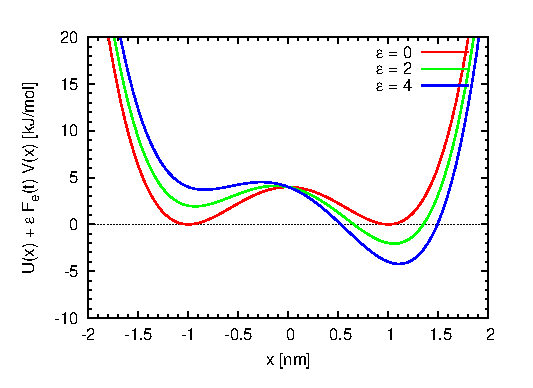
\includegraphics[width=0.4\textwidth]{figs/fig-tilt-pot.eps}
  \caption{The double-well potential with tilting perturbation.}
  \label{fig:tmp1}
\end{figure}

We test the idea firstly by a one-dimensional model system: one particle in a
tilting double-well potential. For convenience, we let the mass of the
particle to be 1 \textsf{amu}. The unperturbed
Hamiltonian of the system is given by:
\begin{align}
  \mh (\vect p, \vect q) = \frac 12 \vect p^2 + U(\vect q) 
\end{align}
with potential
\begin{align}
  U(\vect q) = \frac12 k (\vect q^2 - a^2)^2
\end{align}
Here $k = 8$~$\textsf{kJ} / (\textsf{mol nm}^4)$, and $ a = 1\ \textsf{nm}$.
Notice at room temperature $300\ \textsf{K}$, $k_BT = 2.48$~\textsf{kJ/mol}.
See the red line in Fig.~\ref{fig:tmp1}.
%$\textsf{kJ} / (\textsf{mol nm}^4)}$
The perturbation is given by
\begin{align}
  \vect C(\vect p, \vect q) = 0; \qquad
  \vect D(\vect p, \vect q) = -\nabla_{\vect q} V(\vect q) = 1
\end{align}
Here $V(\vect q) = -\vect q$ is  effectively tilt the original
potential $U(\vect q)$. The strength of the perturbation $F_e(t)$ is given
by the following function:
\begin{align}
  F_e(t) = 
  \begin{cases}
    F_e^{\textrm{max}}\times (t / t_c) & t < t_c \\
    F_e^{\textrm{max}} & t \geq t_c
  \end{cases}
\end{align}
$t_c = 20$~\textsf{ps} so that the perturbation increases slow
enough: the typical decaying time scale of the correlation function
in~\eqref{eqn:core-identify-approx-2} is roughly 3~\textsf{ps}.
We choose $\tau = 1$~\textsf{ps}.
% We choose $\mt_\alpha$
% to be the propagator of the Langevin dynamics at temperature $150$
% \textsf{K} with $\alpha = 1$ \textsf{ps}.
Since the dynamics is in
1-d, the projection $\mathcal P$ is identity.  We consider the stability of the
distribution $f(\vect x, t)$ at time $t$: $\Delta\mt_\tau f(\vect x, t)$.
The larger
this value, the more stable the core sets are.

See Fig. \ref{fig:tmp2} and \ref{fig:tmp3} for numerical result.  Both
the direct non-equilibrium simulation and the linear response
approximation are presented. Time slices $t = 0$, 10, 15 and 20
\textsf{ps} are shown.  When the perturbation is small,
i.e. $F_e^{\textrm{max}} = 2$, the direct non-equilibrium simulation
and the linear response results are accurately consistent. As the
perturbation grows stronger, the left well becomes less stable, while
the right well becomes more stable.  When the perturbation is big,
i.e. $F_e^{\textrm{max}} = 4$, the linear response results are no
longer precise. When $t\geq 10$ \textsf{ps}, the left well basically
disappears, however, the linear response calculation presents
artifical occilation at the right well.

\begin{figure}
  \centering
  \includegraphics[width=0.95\textwidth]
  {figs/tilt.warm020.str2.0.nst1e09.smallgrid/fig-2d.eps}
  \caption{The plot of $\Delta\mt_\tau f(\vect x,t)$  under perturbation of
    $F_e^{\textrm{max}} = 2$.
    Upper row: the direct non-equilibrium simulation. Lower row: the
    results of linear response formula~\eqref{eqn:core-identify-approx-2}.
  }
  \label{fig:tmp2}
\end{figure}

\begin{figure}
  \centering
  \includegraphics[width=0.95\textwidth]
  {figs/tilt.warm020.str4.0.nst1e09.smallgrid/fig-2d.eps}
  \caption{The plot of $\Delta\mt_\tau f(\vect x,t)$  under perturbation of
    $F_e^{\textrm{max}} = 4$.  Upper row: the direct non-equilibrium
    simulation. Lower row: the results of linear response
    formula~\eqref{eqn:core-identify-approx-2}.  }
  \label{fig:tmp3}
\end{figure}


\subsection{Splitting single-well potential}

\begin{figure}
  \centering
  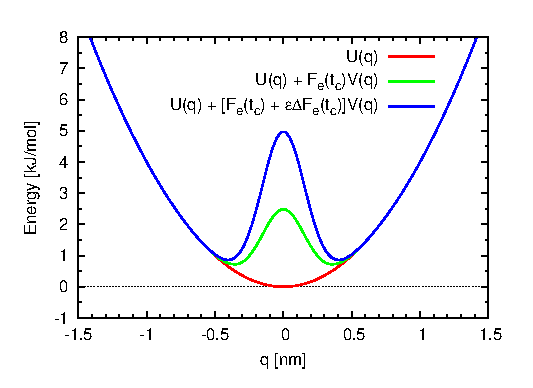
\includegraphics[width=0.4\textwidth]{figs/fig-split-pot.eps}
  \caption{The single-well potential with splitting perturbation.}
  \label{fig:tmp4}
\end{figure}

In this splitting single-well potential example, the unperturbed
potential is simply the harmonic potential given by:
\begin{align}
  U(\vect q) = \frac12\,k\,\vect q^2 
\end{align}
Here $k = 8$~$\textsf{kJ} / (\textsf{mol nm}^2)$.
Notice at room temperature $300\ \textsf{K}$, $k_BT = 2.48$~\textsf{kJ/mol}.
See the red line in Fig.~\ref{fig:tmp4}.
%$\textsf{kJ} / (\textsf{mol nm}^4)}$
The perturbation is again given by
\begin{align}
  \vect C(\vect p, \vect q) = 0; \qquad
  \vect D(\vect p, \vect q) = -\nabla_{\vect q} V(\vect q) 
\end{align}
where $V(\vect q)$ is a Gaussian type potential:
\begin{align}
  V(\vect q) = \frac{1}{\sqrt{2\pi \sigma^2}}
  \exp\Big\{-\frac{\vect q^2}{2\sigma^2}\Big\}
\end{align}
we use $\sigma = 0.16$~\textsf{nm}. Please see Fig~\ref{fig:tmp4}.
For the results, please see Fig.~\ref{fig:tmp5} -- Fig.~\ref{fig:tmp6}.
\begin{figure}
  \centering
  \includegraphics[width=0.95\textwidth]
  {figs/split.warm020.str1.0.nst1e09.smallgrid.more/fig-2d.eps}
  \caption{The plot of $\Delta\mt_\tau f(\vect x,t)$  under perturbation of
    $F_e^{\textrm{max}} = 1.0$.
    Upper row: the direct non-equilibrium simulation. Lower row: the
    results of linear response formula~\eqref{eqn:core-identify-approx-2}.
  }
  \label{fig:tmp5}
\end{figure}

\begin{figure}
  \centering
  \includegraphics[width=0.95\textwidth]
  {figs/split.warm020.str2.0.nst1e09.smallgrid.more/fig-2d.eps}
  \caption{The plot of $\Delta\mt_\tau f(\vect x,t)$  under perturbation of
    $F_e^{\textrm{max}} = 2.0$.  Upper row: the direct non-equilibrium
    simulation. Lower row: the results of linear response
    formula~\eqref{eqn:core-identify-approx-2}.  }
  \label{fig:tmp6}
\end{figure}



\section{Non-equilibrium linear response}

% \subsection{Path integral}
% The path integral is very useful to develop the non-equilibrium version of
% linear response theory. 
% Comparing with the idea of ensemble, which is a collection of state points
% in the configuration space, the path integral consider the ``ensemble'' of
% trajectories.
% (In the following, the develop of formula are formal. The strict mathematical
% theory is still unclear for me.)
% First, we take the standard 1-dimensional Wiener process for example.
% Consider the time interval $[0,T]$, the probability density of one trajectory
% is given by
% \begin{align}
%   p[W_t] = \frac 1Z e^{-I[W_t]}
% \end{align}
% where $I$ is the action functional of Wiener process given by
% \begin{align}
%   I[W_t] = \int_0^T\frac12 \dot{W}_t^2\dd t
% \end{align}
% the partition function $Z$ is
% \begin{align}
%   Z = \int  e^{-I[W_t]} \prod_{0\leq t\leq T}\dd W_t
% \end{align}
% Consider the following two stochastic processes:
% \begin{align}\label{eqn:st-orig}
%   \dd \vect X_t &= \vect b(\vect X_t, t) \dd t + \bsigma(\vect X_t, t)\,\dd\vect W_t \\\label{eqn:st-pert}
%   \dd \vect Y_t &= \vect b(\vect Y_t, t) \dd t + \vect c(\vect Y_t, t) \dd t + \bsigma(\vect Y_t, t)\,\dd\vect W_t
% \end{align}
% Where $\vect W_t$ is the standard Wiener process. Obviously
% \eqref{eqn:st-pert} is the perturbed version of
% \eqref{eqn:st-orig}. It has been shown that, starting from the same
% measure saying $\mu$ (which is not necessarily equilibrium or
% stationary), the ratio of trajectory probability density between the perturbed
% and unperturbed process is~\cite{li2010lecture} (\recheck{I think here
%   the incompressibility of phase space should be assumed. Otherwise the
%   ratio should be more complicated.})
% \begin{align}\label{eqn:girsanov}
%   \frac{\dd\mathcal P_{\vect Y}}{\dd\mathcal P_{\vect X}}
%   =
%   \exp
%   \Big\{
%   -\frac12 \int_0^T\vert\bsigma^{-1}\cdot\vect c(\vect X_t,t)\vert^2\,\dd t
%   +\int_0^T[\dot{\vect X}_t - \vect b(\vect X_t,t)]^T
%   \cdot\bsigma^{-T}\cdot\bsigma^{-1}\cdot\vect c(\vect X_t,t)\,\dd t 
%   \Big\}
% \end{align}
% where $\mathcal P_{\vect Y}$ and $\mathcal P_{\vect Y}$ are measures
% of the trajectories generated by \eqref{eqn:st-pert} and
% \eqref{eqn:st-orig}, respectively.  This result (Girsanov formula?) is
% (formally) precise without any approximation.


\subsection{Non-equilibrium perturbation with linear approximation}

To be more general, we study the two perturbed Langevin dynamics
(i.e. Eqn.~\eqref{eqn:langevin-1} and \eqref{eqn:langevin-2}) with
different perturbations that are given by $F_e^1(t)$ and $F_e^2(t)$,
respectively. We consider the difference between the observations of
these dynamics:
\begin{align}\label{eqn:noneq-pert-1}
  \langle Q(t)\rangle_{\mu}^{2}  -\langle Q(t)\rangle_{\mu}^{1}
  &=
  \int Q(\vect X_t) \,\dd\mathcal P^2[\vect X_t]
  -\int Q(\vect X_t) \,\dd\mathcal P^1[\vect X_t]
  =
  \int Q(\vect X_t)
  \Big\{
  \frac{\dd\mathcal P^2[\vect X_t]}{\dd\mathcal P^1[\vect X_t]}
  -1
  \Big\}
  \,\dd\mathcal P^1[\vect X_t]
\end{align}
\recheck{Here we further assume that $\vect C(\vect q, \vect p) = 0$.
  (otherwise the Girsanov formula~\eqref{eqn:girsanov} may be unstable...
  By letting the $\epsilon$ in the following formula to 0, if
  $\vect C\neq 0$, the limit may not be exist. This
  is intuitionally not likely... I do not know why.)}
By writing Eqn.~\eqref{eqn:langevin-1} and \eqref{eqn:langevin-2} as
\begin{align}
  \frac{\dd }{\dd t}
  \left[
    \begin{array}{l}
      \vect q\\
      \vect p
    \end{array}
  \right]
  =
  \left[
    \begin{array}{l}
      \nabla_{\vect p}\mh\\
      -\nabla_{\vect q}\mh - \gamma\vect p + F_e\vect D
    \end{array}
  \right]
  \dd t
  +
  \left[
    \begin{array}{cc}
      \epsilon \vect I & 0\\
      0 & \sigma\vect I
    \end{array}
  \right]
  \cdot
  \left[
    \begin{array}{l}
      \dd\vect W_t\\
      \dd\vect W_t
    \end{array}
  \right]
\end{align}
Using Girsanov's formula, to the leading order of $\Delta F_e = F_e^2 - F_e^1$,
we have
\begin{align}\nonumber
  \frac{\dd\mathcal P^2[\vect X_t]}{\dd\mathcal P^1[\vect X_t]}
  -1
  &=
  \exp
  \Big\{
  \frac 1 {\sigma^2}
  \int_0^t
  [\dot{\vect p}_s +
  \gamma\vect p_s +
  \nabla_{\vect q}\mh(\vect q_s,\vect p_s)
  - F_e^1(s) \vect D(\vect q_s,\vect p_s)
  ]\cdot
  \vect D(\vect q_s,\vect p_s)
  \Delta F_e(s)\,
  \dd s
  + \mathcal O(\Delta F_e^2)
  \Big\} - 1 \\\label{eqn:girsanov-langevin-1}
  &\approx
  \frac 1 {\sigma^2}
  \int_0^t
  [\dot{\vect p}_s +
  \gamma\vect p_s +
  \nabla_{\vect q}\mh(\vect q_s,\vect p_s)
  - F_e^1(s) \vect D(\vect q_s,\vect p_s)
  ]\cdot
  \vect D(\vect q_s,\vect p_s)
  \Delta F_e(s)\,
  \dd s  
\end{align}
This is where the \emph{linear approximation} applies.
By using the relation $\beta = 2\gamma / \sigma^2$ and split the
Eqn.~\eqref{eqn:girsanov-langevin-1} into time symmetric and
antisymmetric parts~\cite{baiesi2010nonequilibrium2}, we have:
\begin{align}\nonumber
  \frac{\dd\mathcal P^2[\vect X_t]}{\dd\mathcal P^1[\vect X_t]}
  -1
  \approx& \:
  \frac\beta 2
  \int_0^t
  \Delta F_e(s)\,
  \vect p_s\cdot \vect D(\vect q_s,\vect p_s)\,
  \dd s\\  \label{eqn:girsanov-langevin-2}
  &\,-
  \frac 1{\sigma^2}
  \int_0^t
  \Delta F_e(s)\,
  \vect F^1(\vect q_s,\vect p_s)\cdot \vect D(\vect q_s,\vect p_s)\,
  \dd s  
  +
  \frac 1{\sigma^2}
  \int_0^t
  \Delta F_e(s) \vect D(\vect q_s,\vect p_s)\cdot \dd \vect p_s,
\end{align}
where $\vect F^1(\vect q_s,\vect p_s) = -\nabla_{\vect q}\mh(\vect
q_s,\vect p_s) + F_e^1(t) \vect D(\vect q_s,\vect p_s)$.  The first
line of the r.h.s. of Eqn.~\eqref{eqn:girsanov-langevin-2} is the time
integrated excess entropy flux, which is time-antisymmetric, while the
second line is the excess dynamic activity that is time-symmetric.
Inserting Eqn.~\eqref{eqn:girsanov-langevin-2} into
\eqref{eqn:noneq-pert-1}, we have
\begin{align}\nonumber
  \langle O(t)\rangle_{\mu}^{2}  -\langle O(t)\rangle_{\mu}^{1}
  =&\,
  \frac\beta 2
  \int_0^t\dd s\,
  \Delta F_e(s)\,
  \big\langle
  \vect p_s\cdot\vect D(\vect X_s)\,O(\vect X_t)
  \big\rangle_\mu^1 \\  \label{eqn:noneq-pert-2}
  &
  -
  \frac1{\sigma^2}
  \int_0^t\dd s\,
  \Delta F_e(s)\,
  \big\langle
  \vect F^1(\vect X_s)\cdot\vect D(\vect X_s)\,O(\vect X_t)
  \big\rangle_\mu^1
  +
  \frac1{\sigma^2}
  \int_0^t
  \Delta F_e(s)\,
  \big\langle
  \dd \vect p_s\cdot\,
  \vect D(\vect X_s)\,O(\vect X_t)
  \big\rangle_\mu^1  
\end{align}
If $\vect D(\vect x)$ is independent of momentum and is conservative,
saying $\vect D(\vect x) = \vect D(\vect q) = -\nabla_{\vect q}
V(\vect q)$, then the last term of \eqref{eqn:noneq-pert-2} can be
further simplified, because
\begin{align}
  -\dd\, [\nabla_{\vect q}V(\vect q_s)\cdot \vect p_s]
  =
  -\nabla_{\vect q}V(\vect q_s)\cdot\dd \vect p_s
  - \vect p_s\cdot\nabla^2_{\vect q}V(\vect q_s)\cdot\vect p_s\,\dd s,
\end{align}
then \eqref{eqn:noneq-pert-2} changes to
\begin{align}\nonumber
  \langle O(t)\rangle_{\mu}^{2}  -\langle O(t)\rangle_{\mu}^{1}
  =&\,
  -\frac\beta 2
  \int_0^t\dd s\,
  \Delta F_e(s)\,
  \big\langle
  \vect p_s\cdot\nabla_{\vect q} V(\vect X_s)\,O(\vect X_t)
  \big\rangle_\mu^1 \\\nonumber
  & +
  \frac1{\sigma^2}
  \int_0^t\dd s\,
  \Delta F_e(s)\,
  \big\langle
  \vect F^1(\vect X_s)
  \cdot\nabla_{\vect q} V(\vect X_s)
  \,O(\vect X_t)
  \big\rangle_\mu^1 \\\nonumber
  & -
  \frac1{\sigma^2}
  \int_0^t
  \dd s\,
  \Delta F_e(s)\,
  \frac{\dd}{\dd s}
  \big\langle
  \vect p_s\cdot\,
  \nabla_{\vect q} V(\vect X_s)
  \,O(\vect X_t)
  \big\rangle_\mu^1    \\\label{eqn:noneq-pert-3}
  & +
  \frac1{\sigma^2}
  \int_0^t
  \dd s\,
  \Delta F_e(s)\,
  \big\langle
  \vect p_s\vect p_s:
  \nabla^2_{\vect q} V(\vect X_s)
  \,O(\vect X_t)
  \big\rangle_\mu^1      
\end{align}


\subsection{Remarks and possibilities}
\bluec{
\begin{itemize}
\item It can be shown that 
  Eqn.~\eqref{eqn:noneq-pert-3} simply reduces to
  \eqref{eqn:eqi-pert-1}
  in the equilibrium case~\cite{baiesi2010nonequilibrium2}.
\item  Eqn.~\eqref{eqn:noneq-pert-3} shows that the trajectory average of
  $F_e^2$ is calculated from the trajectory average of $F_e^1$. We
  assume: (1) they start from the same initial distribution $\mu$, and
  (2) $F_e^2$ is not very far from $F_e^1$ so that the linear
  approximation is reasonably valid.  The condition (1) can be made
  weaker, for example $F_e^2$ starts from $\mu_2$ and $F_e^1$ starts
  from $\mu_1$, however, $\mu_2$ should be similar to $\mu_1$,
  otherwise the sampling is of poor accuracy.
  (2) means all possible trajectories of perturbation $F_e^2$ should be
  effciently sampled by perturbation $F_e^1$.
\item Eqn.~\eqref{eqn:noneq-pert-3}, may be used in this way:
  assume we want to study the dynamics of $F_e^2$, which is very slow
  and difficult to handle directly.
  We can instead study the dynamics of $F_e^1$, which is
  similar to $F_e^2$, but is much faster, so that it can be handle by MD.
  And then use \eqref{eqn:noneq-pert-3} to calculate the averages of
  the target dynamics $F_e^2$.
  A possible choice of  $F_e^1$ may be  $F_e^1 = \alpha F_e^2,\ \alpha > 1$.
  On the other hand, perturbation $F_e^2$ should be not very far
  from $F_e^1$, that means $F_e^2$ can not arbitrarily accelerate
  $F_e^1$. Fortunately we have the freedom to design $F_e^2$, therefore,
  an error estimate may help, and a path optimization of $F_e^2$
  may be developed.
\item The perturbation $F_e^1$ can be kept a constant so that the
  system reaches a stationary state.
  $F_e^2$ is perturbation from that stationary state.
  The averages in
  \eqref{eqn:noneq-pert-3} can be calculated easier, because
  what we sample is the stationary state, rather the trajectories.
  When the system is far from the stationary state, the
  accuracy is low. 
\item It may also be possible to study multiple reference dynamics,
  and use interpolations to increase the accuracy of the linear
  approximation.
\item Extension to nonlinear response?
\end{itemize}
}









\section*{References}
\bibliography{ref}{}
\bibliographystyle{unsrt}





\end{document}